% !TeX root = ../main.tex
\chapter{Introduction}
This chapter will first introduce Explainable AI and why it is very important in autonomous driving. Then, multi-modal 3D object detection is described. Finally, an overview of the transformer architecture is described. 

\section{Explainable AI}
Artificial intelligence is now an indispensable tool which enhances our life quality.
Due to the increasing complexity of state-of-the-art deep learning models, the AI models are often viewed as a "black box" where only the inputs and the predictions are visualized. This leads to the problem of "trusting" the AI without understanding how it works, as can be seen in Figure \ref{fig:accvsexpl}. Thus, it is becoming more and more important to understand why and how a model reached a certain decision. This is expecially important when the safety of people depends by the AI, such as in healthcare and automotive driving \cite{abeloos2022explaining}.
The techniques used to explain the predictions made by the AI and make them more interpretable are referred to as Explainable AI (XAI). The objective of XAI is to eliminate the "black-box" models by explaining its behavior.
It not only enhances security and trustiness for the end-user, but it also helps the developer to improve the model, for example by removing potential biases. In fact, consider an example in which an object detection model has very good performance metrics. If the dataset contained objects with a specific background, e.g a golf ball with grass as background, then it is highly possible that the model is biased. In that case, it could mistakenly detect a golf ball each time there is grass as background. Through XAI, the developer could easily identify this bias and correct it.
The more explainable a model is, the easier it becomes to improve it. 
XAI could solve security problems: adversarial attacks can mislead an object detector to confuse one image with another just by changing some pixels, leading to unintended behaviors. This is particular critical in automoted driving. Those important pixels attributed by the model could be identified by XAI.
In case of accidents, XAI could help identify the cause, thus improving accountability.
\begin{figure}[h]
    \centering
    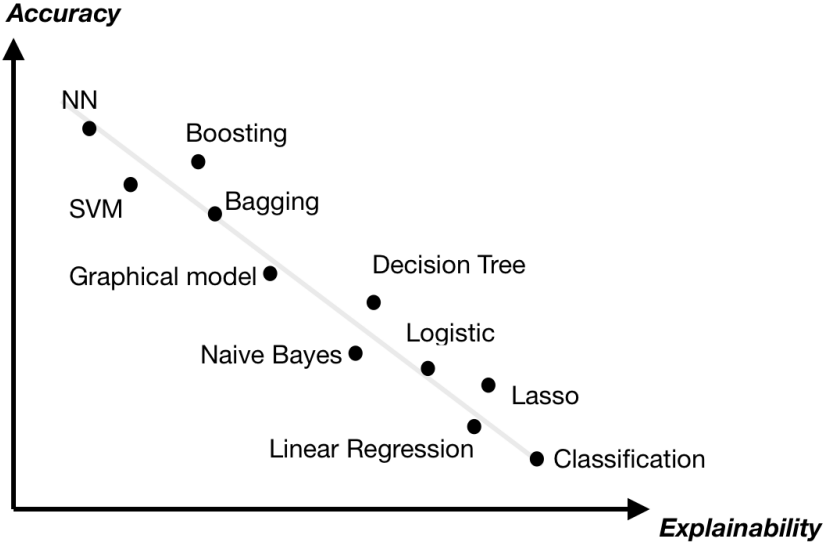
\includegraphics[scale=0.4]{accvsexpl-duval2019explainable}
    \caption{Accuracy vs Explainability of the main machine learning algorithms \cite{duval2019explainable}}
    \label{fig:accvsexpl}
    \end{figure}


\section{Multi-Modal 3D Object Detection}
Autonomous driving is progressing towards self-driving cars thanks to the advanced machine learning models. One of the main difficulties is due to the complex and dynamic driving environment, which require a sofisticated artificial vision \cite{wang2021multi}. Object detection aims to identify the objects in the scene, their location and category \cite{wang2021multi}. Perception with a single modality suffers some drawbacks, such as difficulties on detecting occluded and large objects \cite{huang2022multi}\cite{caesar2020nuscenes}. Equipping the car with more sensors (multi-modal) improves accuracy and robustness. LiDAR (Light Detection and Ranging) sensor contains accurate localization in 3D, while cameras allow measurements of color and edges \cite{caesar2020nuscenes}. It is becoming common to fuse data from LiDAR and cameras for better performance instead of using them separately, but this approach requires precise synchronization.
The success of 2D object detection has been unprecedented thanks to the development of deep learning-based models like RCNN, Fast RCNN, and Faster R-CNN. However, 2D detection can only provide limited information such as the 2D bounding box of an object, which is not enough for autonomous vehicles to perceive their environment. Thus, 3D object detection has become a more challenging but crucial task as it helps with more accurate spatial path planning and navigation. In this task, more output parameters are required to specify the 3D-oriented bounding boxes around objects \cite{wang2021multi}.

% TO-ADD: different types of multi-modal 3D object detection and architectures


\section{Transformers}
%Describe Transformer architecture and its usage in visual applications
Transformers have become the standard machine learning model in natural language processing (NLP) \cite{dosovitskiy2020image}. They were introduced in 2017 by a team at Google Brain \cite{Att.2017} as fully attention-based model. The attention mechanism was invented in 2014 to address some problems arising in Recurrent Neural Networks (RNN) in machine translation \cite{bahdanau2014neural}. For instance, RNNs suffer with long text and slow training. The attention mechanism was then implemented by RNN-based encoder-decoder architectures to solve those problems. However, these models still rely on recurrence, which is incompatible with parallel computation. Transformers get rid of recurrence and convolutions and are based only on attention mechanism \cite{Att.2017}. Thanks to their efficiency, Transformer models are trained with unprecedented size \cite{dosovitskiy2020image}. Attentions perform global computation which made them applicable in NLP and, recently, in computer vision. To appreciate how Trasformers revolutionized the AI world, an understanding of the attention mechanism is needed.

\subsection{Attention}
Suppose we have the sentence \emph{"Mark eats an apple while he is going to the gym"}. It is composed of 11 words or tokens. Considering the word \emph{he}, it more related to the word \emph{Mark} instead of \emph{apple}, even if the latter is closer to the word \emph{Mark}. Context, therefore, is more important than proximity. The idea of \emph{self-attention}, in this case, is to figure out how important all the other words in the sentence are with respect to a specific word, without any recurrent connections. It is based on just weighted sums and activations, so they can be very parallelizable and efficient. If this sentence needs to be translated, to German for example, then the output text can interact with the input through \emph{cross-attention}.
In the case of object detection, tokens can represent feature patches of an image. For instance, an image is divided into a sequence of patches \cite{dosovitskiy2020image}\cite{carion2020end}. This is one big advantage of Transformers, i.e they can handle different data types (text, image and sound).
To allow the attention mechanism to learn patterns and improve context, trainable parameters are needed: \emph{Query}, \emph{Key} and \emph{Values} are the main components. Each token is projected to its own query,key and value by three different weight matrices, which are learnt during training. Those are used to calculate the \emph{attention scores}:
\begin{equation}
    Attention(\emph{Q,K,V}) = softmax(\frac{\emph{\textbf{Q}} \cdot \emph{\textbf{K}}^T}{\sqrt{d_{k}}}) \cdot V
\end{equation}


\subsection{Positional encoding}
...
\subsection{Multi-head attention}
...


Figure \ref{fig:transf-arch} shows the Transformer model as depicted in the original paper \cite{Att.2017}. It is composed of an encoder and a decoder, as depicted in the left and right side, respectively. The encoder and the decoder are composed of a stack of \emph{N} layers. Some Transformer architectures are encoder-only or decoder-only. The SpatialDETR, for instance, is a decoder-only architecture \cite{doll2022spatialdetr}.

\begin{figure}[h]
    \centering
    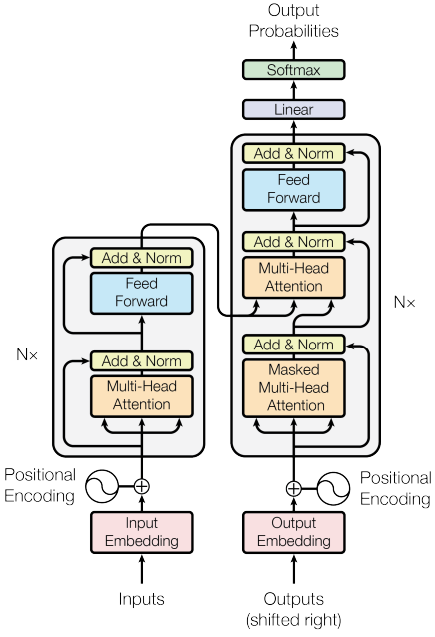
\includegraphics[scale=0.4]{transf-arch}
    \caption{The Transformer model architecture. \cite{Att.2017}}
    \label{fig:transf-arch}
    \end{figure}


%explain transformers, advantage of set-based prediction without nms in detr, problem of training time of detr, deformable detr and detr3d solution to attend only to object center. then explain that spatialdetr allows for a more global attention for objects between cameras. explain decoder-only transformer


    


